% !TeX root = ../../../main.tex
\subsection{Additional Performance Analysis}\label{ch06:apd:add-perf}
Here we report performance plots for the \texttt{sepsis-40} ablation analysis and the i2m4 dataset (main analysis and ablation), analogous to Figure \ref{ch06:fig:time-disc}. Figure \ref{ch06:fig:sep40ablate-time-disc} displays the performance of the Llama 3.3 ablations on \texttt{sepsis-40}.  In terms of match rate, the ablations perform within 5 percent of each other except for the 0-shot and Interval plus Typing (Int+Type) methods.  In the temporal assessment figures we see that, for example, the 0-shot method shows promising temporal performance characteristics, but recall that it suffers from much lower event match rates. The Interval plus Typing method (Int+Type) shows a similar pattern.  Requesting the interval alone (Interval) results in worse time discrepancy characteristics as compared to the main approach.  


% !TeX root = ../../../main.tex
\begin{figure}[htbp]
\begin{ChSixFloatBody}

\centering
    \begin{minipage}[t]{0.30\textwidth}
    \centering
    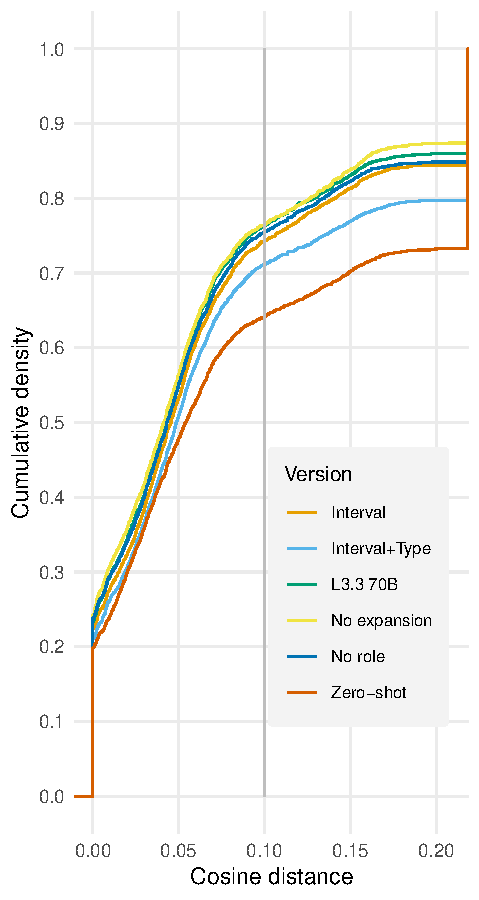
\includegraphics[width=\linewidth, page=1]{Appendices/appendix-ch06/images/figures/main_results_figures/figures_sepsis_40_ablations.pdf}
    \end{minipage}
% \end{figure}
    % \hfill
    \begin{minipage}[t]{0.30\textwidth}
% \begin{figure}[h!]j
    \centering
    \includegraphics[width=\linewidth, page=2]{Appendices/appendix-ch06/images/figures/main_results_figures/figures_sepsis_40_ablations.pdf}
    \end{minipage}
    % \caption{Event match cumulative distribution function (left) and  concordance box-plots (right) for the \texttt{sepsis-40} dataset.}
    % \label{fig:sep10eventc}
% \end{figure}
% \begin{figure}[tb!]

    \begin{minipage}[t]{0.30\textwidth}
    \centering
    \includegraphics[width=\linewidth, page=3]{Appendices/appendix-ch06/images/figures/main_results_figures/figures_sepsis_40_ablations.pdf}
    \end{minipage}
% \end{figure}
% \begin{figure}[h!]
    \begin{minipage}[t]{0.30\textwidth}
    \centering
    \includegraphics[width=\linewidth, page=4]{Appendices/appendix-ch06/images/figures/main_results_figures/figures_sepsis_40_ablations.pdf}
    \end{minipage}
    
    

\end{ChSixFloatBody}
\caption{Event match cumulative distribution function (top left) and  concordance box-plots (top right) for the \texttt{sepsis-40} ablations. 
    Time discrepancy from the manual annotation timestamps among matched events, overall (bottom left) and disaggregated by clinician annotator timestamp (time from presentation, bottom right).}\ChSixFloatLabel{ch06:fig:sep40ablate-time-disc}
\end{figure}


Figures \ref{ch06:fig:i2m4-time-disc} and \ref{ch06:fig:i2m4ablate-time-disc} displays the performance of the models and the Llama 3.3 ablations on the i2m4 dataset.  The match rates and concordances are visibly lower in the i2m4 dataset than in \texttt{sepsis-40}. Comparing across methods, Llama 3.3 visibly outperforms the Llama 3.1 models in both measures.
Despite the lower match rates and concordances, the time discrepancies in i2m4 were comparatively stronger (AULTC of 0.703). In terms of time discrepancy, Llama 3.1 70B demonstrate smaller time discrepancies, but at the cost of an event match rate of only 30 percent.
In the ablation analysis of the i2m4 dataset, we observe that the Interval technique performs very similarly to the Llama 3.3 version (unlike in the \texttt{sepsis-40} dataset, where it underperforms markedly with respect to time discrepancy).


% !TeX root = ../../../main.tex
\begin{figure}[htbp]
\begin{ChSixFloatBody}

\centering
    \begin{minipage}[t]{0.3\textwidth}
    \centering
    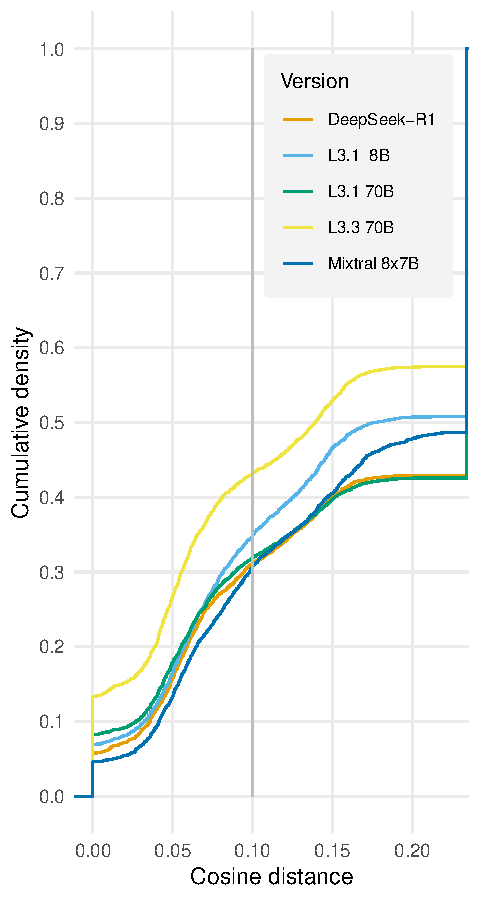
\includegraphics[width=\linewidth, page=1]{Appendices/appendix-ch06/images/figures/main_results_figures/figures_i2m4.pdf}
    \end{minipage}
% \end{figure}
    % \hfill
    \begin{minipage}[t]{0.3\textwidth}
% \begin{figure}[h!]j
    \centering
    \includegraphics[width=\linewidth, page=2]{Appendices/appendix-ch06/images/figures/main_results_figures/figures_i2m4.pdf}
    \end{minipage}
    % \caption{Event match cumulative distribution function (left) and  concordance box-plots (right) for the \texttt{sepsis-40} dataset.}
    % \label{fig:sep10eventc}
% \end{figure}
% \begin{figure}[tb!]

    \begin{minipage}[t]{0.3\textwidth}
    \centering
    \includegraphics[width=\linewidth, page=3]{Appendices/appendix-ch06/images/figures/main_results_figures/figures_i2m4.pdf}
    \end{minipage}
% \end{figure}
% \begin{figure}[h!]
    \begin{minipage}[t]{0.3\textwidth}
    \centering
    \includegraphics[width=\linewidth, page=4]{Appendices/appendix-ch06/images/figures/main_results_figures/figures_i2m4.pdf}
    \end{minipage}
    
    

\end{ChSixFloatBody}
\caption{Event match cumulative distribution function (top left) and  concordance box-plots (top right) for the i2m4 dataset. 
    Time discrepancy from the manual annotation timestamps among matched events, overall (bottom left) and disaggregated by clinician annotator timestamp (time from presentation, bottom right).}\ChSixFloatLabel{ch06:fig:i2m4-time-disc}
\end{figure}



% !TeX root = ../../../main.tex
\begin{figure}[htbp]
\begin{ChSixFloatBody}

\centering
    \begin{minipage}[t]{0.3\textwidth}
    \centering
    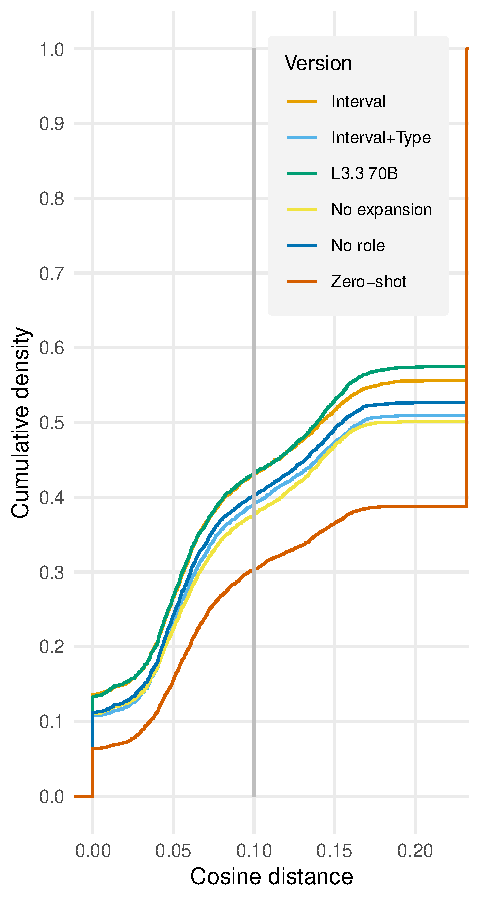
\includegraphics[width=\linewidth, page=1]{Appendices/appendix-ch06/images/figures/main_results_figures/figures_i2m4_ablations.pdf}
    \end{minipage}
% \end{figure}
    % \hfill
    \begin{minipage}[t]{0.3\textwidth}
% \begin{figure}[h!]j
    \centering
    \includegraphics[width=\linewidth, page=2]{Appendices/appendix-ch06/images/figures/main_results_figures/figures_i2m4_ablations.pdf}
    \end{minipage}
    % \caption{Event match cumulative distribution function (left) and  concordance box-plots (right) for the \texttt{sepsis-40} dataset.}
    % \label{fig:sep10eventc}
% \end{figure}
% \begin{figure}[tb!]

    \begin{minipage}[t]{0.3\textwidth}
    \centering
    \includegraphics[width=\linewidth, page=3]{Appendices/appendix-ch06/images/figures/main_results_figures/figures_i2m4_ablations.pdf}
    \end{minipage}
% \end{figure}
% \begin{figure}[h!]
    \begin{minipage}[t]{0.3\textwidth}
    \centering
    \includegraphics[width=\linewidth, page=4]{Appendices/appendix-ch06/images/figures/main_results_figures/figures_i2m4_ablations.pdf}
    \end{minipage}
    
    

\end{ChSixFloatBody}
\caption{Event match cumulative distribution function (top left) and  concordance box-plots (top right) for the i2m4 ablations. 
    Time discrepancy from the manual annotation timestamps among matched events, overall (bottom left) and disaggregated by clinician annotator timestamp (time from presentation, bottom right).}\ChSixFloatLabel{ch06:fig:i2m4ablate-time-disc}
\end{figure}

% This is the second appendix.




\FloatBarrier
